\documentclass[11pt,a4paper]{article}

% ── Packages ──────────────────────────────────────────────────────────
\usepackage[utf8]{inputenc}
\usepackage[T1]{fontenc}
\usepackage{lmodern}
\usepackage[margin=2.5cm]{geometry}
\usepackage{amsmath,amssymb,amsthm}
\usepackage{booktabs}
\usepackage{graphicx}
\usepackage{hyperref}
\usepackage{xcolor}
\usepackage{listings}
\usepackage{enumitem}
\usepackage{microtype}
\usepackage{caption}
\usepackage{float}
\usepackage{tikz}
\usetikzlibrary{arrows.meta, positioning, fit, calc}

\hypersetup{
  colorlinks=true,
  linkcolor=blue!60!black,
  citecolor=blue!60!black,
  urlcolor=blue!60!black,
}

% ── Code listings ─────────────────────────────────────────────────────
\definecolor{codebg}{RGB}{248,248,248}
\definecolor{codeframe}{RGB}{200,200,200}
\definecolor{keyword}{RGB}{0,100,170}
\definecolor{string}{RGB}{170,55,0}
\definecolor{comment}{RGB}{100,130,100}

\lstset{
  backgroundcolor=\color{codebg},
  frame=single,
  rulecolor=\color{codeframe},
  basicstyle=\ttfamily\small,
  keywordstyle=\color{keyword}\bfseries,
  stringstyle=\color{string},
  commentstyle=\color{comment}\itshape,
  breaklines=true,
  breakatwhitespace=true,
  tabsize=4,
  showstringspaces=false,
  xleftmargin=1em,
  xrightmargin=1em,
  aboveskip=1em,
  belowskip=1em,
}

\lstdefinelanguage{Rust}{
  morekeywords={fn,let,mut,if,else,for,in,loop,break,continue,return,
    pub,struct,enum,impl,self,Self,use,mod,async,await,move,
    match,Some,None,Ok,Err,true,false,Box,Arc,Vec,String,
    format,println,eprintln},
  morestring=[b]",
  morecomment=[l]{//},
  morecomment=[s]{/*}{*/},
  sensitive=true,
}

% ── Title ─────────────────────────────────────────────────────────────
\title{%
  \textbf{Measured Forgetting:}\\[0.3em]
  \Large Context Management for Agentic Local LLMs%
}
\author{%
  Barak Achillah Asidi\\
  CIF AI\\
  \texttt{thexi.dev}\\
  \texttt{research@thexi.dev}%
}
\date{May 2026}

% ══════════════════════════════════════════════════════════════════════
\begin{document}
\maketitle

% ── Abstract ──────────────────────────────────────────────────────────
\begin{abstract}
We present \emph{measured forgetting}, a context management method for local language models performing multi-round tool-calling on consumer hardware. Unlike cloud-hosted APIs with 128K+ context windows, local models on Apple Silicon (8B--14B parameters, 8K--16K context) exhaust their context within 3--4 tool rounds --- each round appends both a model response and a tool result. Existing approaches either impose a fixed round limit (truncating investigation prematurely) or rely on the user to manage context (shifting cognitive load away from the task).

Measured forgetting treats context as a finite resource to be managed \emph{during} inference, not before it. The method monitors context utilisation in real-time, partitions the message history into three zones (pinned, compressible, recent), and invokes the model itself to compress the compressible zone into a summary --- all within the same generation loop. Version 2 extends uniform compression with three novel instruments --- an Influence Equation (multi-dimensional scoring with super-linear $\Phi(B) = B^{1.5}$ resonance), Trace Topology (causal chain preservation), and a Problem Taxonomy (task-class-adaptive compression strategy). Across 7 models from 5 independent families (Alibaba, Mistral, Meta, Google, Microsoft), V2 outperforms V1 on every model tested, with improvements ranging from +0.04 to +0.46 (out of 3.0), and the largest gains on the weakest summarisers.

Combined with a KV-cache-persistent session worker that eliminates redundant prompt re-processing across rounds, the approach enables unbounded tool-calling depth on a 16K context window while maintaining response quality. Both techniques are deployed in production: measured forgetting in a Tauri desktop application (B.app, Qwen3 8B, M4 Mac), and a variant of the compaction protocol in a cloud-hosted chat orchestrator. Code and benchmark harness: \url{https://github.com/cif-ai/measured-forgetting}.
\end{abstract}

\vspace{1em}
\noindent\textbf{Keywords:} context management, local inference, tool-calling agents, KV cache, information theory, influence scoring, problem taxonomy, llama.cpp

% ══════════════════════════════════════════════════════════════════════
\section{The Problem}

\subsection{Agentic loops exhaust context fast}

A local LLM acting as an agent follows a pattern: the user asks a question, the model generates a response containing a tool call, the orchestrator executes the tool, injects the result, and the model generates again. Each round appends two messages (assistant response + tool result), typically 200--800 tokens each. On a 16K context window with a 2K system prompt, the usable budget is $\sim$14K tokens. At 400 tokens per round-trip, context fills in $\sim$17 rounds --- but quality degrades well before that, as attention dilutes across the growing history.

In practice, we observed reliable degradation after 4--5 tool rounds on Qwen3 8B (8K context) and 6--8 rounds on Qwen3.5 9B (16K context). The failure mode is not a crash --- it is \emph{confabulation}. The model starts generating plausible-sounding responses that ignore the tool results, because the relevant data has been pushed too far back in the context.

\subsection{Fixed round limits are the wrong abstraction}

The naive solution --- cap tool rounds at some fixed $N$ --- trades correctness for safety. A fixed limit of $N=5$ rounds may be too many for a simple lookup (wasting tokens on unnecessary rounds) and too few for a complex investigation that requires querying multiple data sources. The appropriate depth is a property of the \emph{task}, not the \emph{system}.

\subsection{KV cache waste compounds the problem}

In a standard llama.cpp inference loop, each generation round re-tokenizes and re-processes the entire prompt from scratch. If the model has made 4 tool calls, round 5 re-processes the system prompt, the user's question, and all 4 prior tool exchanges --- even though those tokens were already processed identically in round 4. On an M4 Mac at $\sim$30 tokens/second prompt processing, re-decoding 8K tokens takes $\sim$4.4 seconds of pure waste.

% ══════════════════════════════════════════════════════════════════════
\section{Measured Forgetting}

\subsection{Core insight}

The method is grounded in a distinction between what the model \emph{is} and what the model has \emph{learned}. The system prompt (identity, instructions, persona) is invariant across rounds --- it must never be compressed. The user's original question is the task anchor --- it pins the investigation's direction. But the intermediate tool exchanges are \emph{learned data}: high-information at the moment of acquisition, but increasingly compressible as the investigation proceeds, because later rounds subsume earlier findings.

This mirrors Shannon's source coding theorem: a sequence of related observations has redundancy that can be compressed without information loss, provided the compression preserves the sufficient statistic.

\subsection{Three-zone partitioning}

At each iteration of the generation loop, the orchestrator checks whether context utilisation has crossed a threshold:

\begin{equation}
T_{\text{compact}} = \frac{3}{4}\,(C - G)
\label{eq:threshold}
\end{equation}

\noindent where $C$ is the context window size and $G = 2048$ is a generation reserve. When \texttt{last\_input\_tokens} $> T_{\text{compact}}$ and the message history has more than 4 messages, compaction fires.

The message history is partitioned into three zones:

\begin{description}[leftmargin=2em, labelindent=1em]
  \item[Zone 1: Pinned] Messages from index 0 through the user's original question (inclusive). Contains the conversation history and the task anchor. Never compressed. Never discarded.
  \item[Zone 2: Compressible] All intermediate tool exchanges: assistant responses containing tool calls, tool results, error messages, follow-up instructions. Compressed into a summary.
  \item[Zone 3: Recent] The last 2 messages (the most recent tool result and instruction). Preserved verbatim --- the model needs fresh context to continue.
\end{description}

\noindent Figure~\ref{fig:zones} illustrates the three-zone partition before and after compaction.

\begin{figure}[H]
\centering
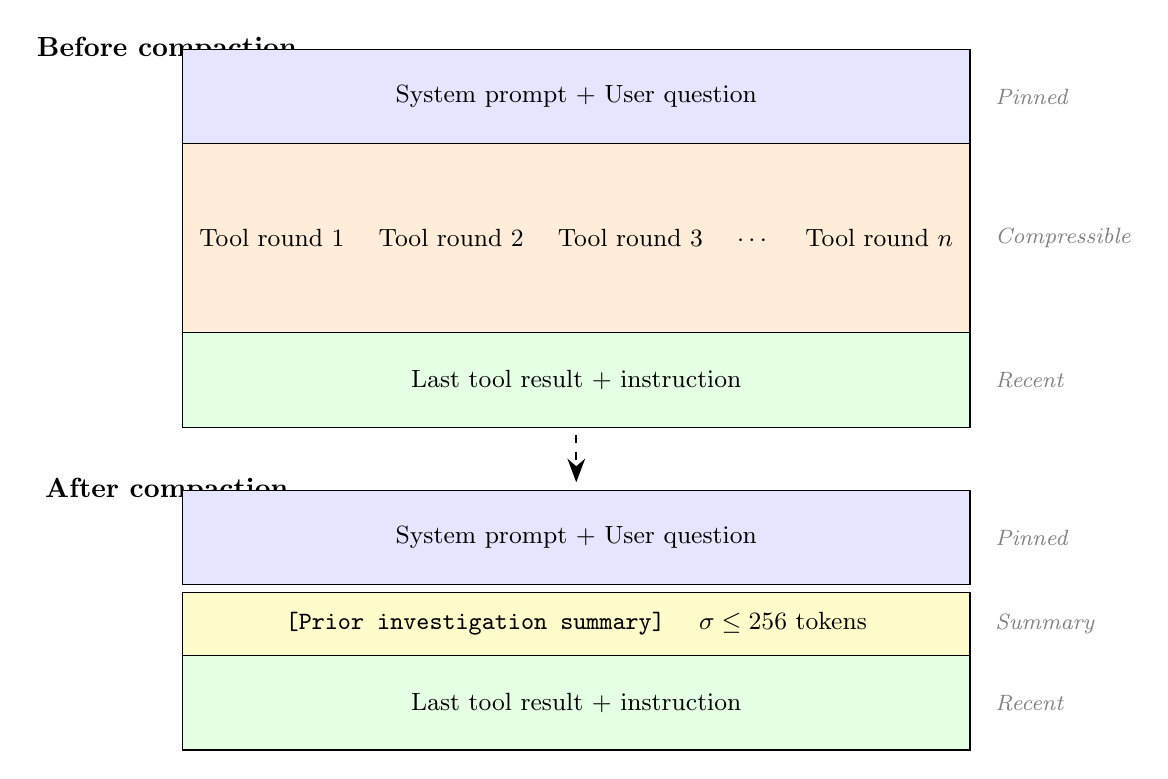
\begin{tikzpicture}[
  zone/.style={draw, minimum width=10cm, minimum height=1.2cm, align=center, font=\small},
  label/.style={font=\footnotesize\itshape, text=gray},
]
  % Before
  \node at (-1.2, 3.6) {\textbf{Before compaction}};
  \node[zone, fill=blue!10] (p1) at (4, 3.0) {System prompt + User question};
  \node[zone, fill=orange!15, minimum height=2.4cm] (c1) at (4, 1.2) {Tool round 1 \quad Tool round 2 \quad Tool round 3 \quad $\cdots$ \quad Tool round $n$};
  \node[zone, fill=green!10] (r1) at (4, -0.6) {Last tool result + instruction};

  \node[label, right] at (9.2, 3.0) {Pinned};
  \node[label, right] at (9.2, 1.2) {Compressible};
  \node[label, right] at (9.2, -0.6) {Recent};

  % After
  \node at (-1.2, -2.0) {\textbf{After compaction}};
  \node[zone, fill=blue!10] (p2) at (4, -2.6) {System prompt + User question};
  \node[zone, fill=yellow!20, minimum height=0.8cm] (s2) at (4, -3.7) {\texttt{[Prior investigation summary]} \quad $\sigma \leq 256$ tokens};
  \node[zone, fill=green!10] (r2) at (4, -4.7) {Last tool result + instruction};

  \node[label, right] at (9.2, -2.6) {Pinned};
  \node[label, right] at (9.2, -3.7) {Summary};
  \node[label, right] at (9.2, -4.7) {Recent};

  % Arrow
  \draw[-{Stealth[length=3mm]}, thick, dashed] (4, -1.3) -- (4, -1.9);
\end{tikzpicture}
\caption{Three-zone partitioning. The compressible zone (potentially thousands of tokens across multiple tool rounds) is replaced by a model-generated summary capped at 256 tokens.}
\label{fig:zones}
\end{figure}

\subsection{Self-summarisation}

The compressible zone is fed to the model itself in a dedicated summarisation pass. The request is deliberately constrained: low temperature (0.2), short output (256 tokens), and explicit instructions to preserve numbers and drop failures:

\begin{lstlisting}[language=Rust, caption={Summarisation request construction}]
let summary_request = InferenceRequest {
    messages: vec![Message {
        role: "user",
        content: format!(
            "Summarize these exchanges into key findings. \
             Bullet points only. Preserve all numbers, data, \
             and facts. Drop failed tool calls:\n\n{}",
            compressible_text
        ),
    }],
    system: "Output only bullet points of key findings. \
             No preamble. No tool calls. No thinking.".into(),
    max_tokens: 256,
    temperature: 0.2,
    top_p: 0.9,
};
\end{lstlisting}

\noindent The result replaces the entire compressible zone. The message array is rebuilt as:

\[
\texttt{messages} = [\,\underbrace{m_0, \ldots, m_q}_{\text{pinned}},\; \underbrace{\sigma}_{\text{summary}},\; \underbrace{m_{n-1}, m_n}_{\text{recent}}\,]
\]

\noindent If summarisation fails (the model produces garbage or times out), the system falls back to hard truncation of the compressible zone to 500 characters --- a lossy but bounded degradation.

\subsection{Error-aware compression}

Not all messages compress equally. Tool errors are aggressively reduced to a single line (the error type), while successful tool results are truncated to 400 characters per message before being fed to the summariser. This differential compression reflects the information content: a successful query result contains data the model needs; a failed query contains only the information ``this approach didn't work.''

\subsection{Dynamic exit conditions}

Measured forgetting v1 eliminates fixed round limits. The generation loop runs until one of three conditions fires:

\begin{enumerate}
  \item \textbf{Loop detection} --- the model repeats a tool call it has already made (same function name + same arguments). This indicates the model is stuck, not making progress. Exit and synthesise from what has been gathered.
  \item \textbf{Consecutive error threshold} --- three consecutive tool errors. The model is unable to find a working approach. Exit and acknowledge the limitation.
  \item \textbf{Context exhaustion post-compaction} --- context is full but too few messages remain to compact further ($\leq 4$ messages after a compaction pass). This is the irreducible minimum.
\end{enumerate}

\noindent None of these are round counts. They are \emph{measurements} of the model's progress and the system's resource state.

% ══════════════════════════════════════════════════════════════════════
\section{Dimension-Aware Compression (v2)}
\label{sec:v2}

Version~1 applies uniform compression: all messages in the compressible zone are treated equally by the summariser. This works, but loses information non-uniformly --- causal chains and high-value data points are compressed at the same rate as error messages and redundant lookups.

Version~2 applies three instruments to make compression \emph{dimension-aware}:

\subsection{Instrument 1: Influence Equation}

Each message $m$ is scored by its influence relative to the task:

\begin{equation}
I(m) = \Phi(B_m) \times \sum_{d} w_d(t) \cdot C_d(m)
\label{eq:influence}
\end{equation}

\noindent where:
\begin{itemize}[nosep]
  \item $C_d(m) \in [0, 1]$ is the convergence of message $m$ on dimension $d$ (data, causal, task-reference, entity, temporal, structural)
  \item $w_d(t)$ is the \emph{susceptibility} of dimension $d$ at time $t$ --- decaying as later messages provide the same type of information ($\lambda = 0.7$ per superseding message)
  \item $B_m = |\{d : C_d(m) > 0\}|$ is the number of active dimensions
  \item $\Phi(B) = B^{1.5}$ is the super-linear \emph{resonance multiplier}
\end{itemize}

The key insight: a message that converges on 4 dimensions is not $4\times$ more valuable than a single-dimension message --- it is $4^{1.5} = 8\times$ more valuable (Equation~\ref{eq:influence}), because multi-dimensional convergence is harder to reconstruct from a summary.

\subsection{Instrument 2: Trace Topology}

Messages form causal chains: tool call $\to$ tool result $\to$ interpretation. These chains are \emph{binding units} --- compressing message B without message A destroys the causal connection. The algorithm detects dependency chains via message ordering and role transitions:

\begin{lstlisting}[language=Rust, caption={Causal chain detection}]
let depends_on = if msg.role == "assistant"
    && prev.content.contains("<tool_result>") {
    Some(prev_index)  // This message interprets the tool result
} else {
    None
};
\end{lstlisting}

\noindent Messages within a causal chain are assigned to the same compression tier --- they are preserved or compressed together, never split.

\subsection{Instrument 3: Problem Taxonomy}

The user's original question is classified into one of six problem classes, each with a different \emph{sufficient statistic}:

\begin{table}[H]
\centering
\begin{tabular}{@{}llp{6.5cm}@{}}
\toprule
\textbf{Class} & \textbf{Sufficient Statistic} & \textbf{Compression Strategy} \\
\midrule
Lookup & The answer & Preserve highest-influence tool result; compress everything else aggressively \\
Multi-hop & The chain & Preserve causal chain topology (A $\to$ B $\to$ C) \\
Exploratory & The success & Compress failures to one line each; preserve successes with full detail \\
Aggregation & The totals & Preserve counts and sums; compress individual data points \\
Contradiction & Both paths & Never heavily compress conflicting data --- both sides are the kernel \\
Temporal & The sequence & Preserve chronological order; include all dates/timestamps \\
\bottomrule
\end{tabular}
\caption{Problem taxonomy and associated compression strategies.}
\label{tab:taxonomy}
\end{table}

\subsection{Three-tier compression plan}

The scored messages are partitioned into three tiers (not to be confused with the three zones):

\begin{enumerate}[nosep]
  \item \textbf{Preserve verbatim}: $I(m) > \text{median}$ AND $B_m \geq 3$ (high-influence, multi-dimensional). These appear verbatim in the final summary.
  \item \textbf{Compress lightly}: Members of causal chains or moderate influence. Truncated to 300 characters and fed to the summariser.
  \item \textbf{Compress heavily}: Low influence, errors, saturated dimensions. Reduced to message type + one line.
\end{enumerate}

\noindent The final context after compaction contains: pinned zone + preserved verbatim content + model-generated summary of compressed content + recent zone. The preserved messages act as ``anchors'' that the model can reference directly, while the summary covers the compressed remainder.

\subsection{$\kappa_d$ Saturation (sw-cap)}

When 3+ messages all provide the same type of information (e.g., repeated errors, or multiple data queries returning similar results), the dimension is \emph{saturated}. The summariser is instructed to collapse saturated dimensions into a single line (``5 errors occurred, type: connection timeout'') rather than preserving each instance.

% ══════════════════════════════════════════════════════════════════════
\section{KV Cache Persistence}

\subsection{The redundancy problem}

In a multi-round tool-calling loop, each round's prompt shares a long common prefix with the previous round's prompt. The system prompt, conversation history, and all prior tool exchanges are identical --- only the latest tool result is new. Yet standard inference re-processes the entire prompt from scratch, because the KV cache is discarded between calls.

\subsection{SessionWorker architecture}

We solve this with a \emph{session worker}: a dedicated thread that owns a \texttt{LlamaContext} (the llama.cpp KV cache) and persists it across generation calls. The worker communicates with the async orchestrator via synchronous channels:

\begin{lstlisting}[language=Rust, caption={SessionWorker channel protocol}]
pub struct SessionWorker {
    tx: mpsc::Sender<WorkerCmd>,
}

enum WorkerCmd {
    Generate {
        request: InferenceRequest,
        on_token: TokenCallback,
        resp_tx: mpsc::Sender<Result<InferenceResponse, String>>,
    },
    ClearCache { resp_tx: mpsc::Sender<()> },
    Stop,
}
\end{lstlisting}

\noindent The worker thread holds mutable state that is unsafe to share across threads (the \texttt{LlamaContext}). By confining it to a single thread and communicating via message-passing, we get the benefits of persistent state without the risks of shared mutability.

\subsection{Prefix matching and incremental decode}

On each \texttt{Generate} command, the worker tokenizes the new prompt and finds the longest common prefix with the previously cached tokens:

\begin{lstlisting}[language=Rust, caption={Prefix matching and KV cache trimming}]
let prefix_len = tokens.iter()
    .zip(cached_tokens.iter())
    .take_while(|(a, b)| a == b)
    .count();

let reused = prefix_len.min(*n_past as usize);
let new_tokens = &tokens[reused..];

if reused < *n_past as usize {
    // Prompt diverged -- trim KV cache from divergence point
    ctx.clear_kv_cache_seq(Some(0), Some(reused as u32), None);
    *n_past = reused as i32;
}
\end{lstlisting}

\noindent Three cases arise:

\begin{enumerate}
  \item \textbf{Extension} ($\texttt{reused} = n_{\text{past}}$): The new prompt is a strict extension of the old. Only the new tokens need decoding. This is the common case in tool-calling loops.
  \item \textbf{Divergence} ($\texttt{reused} < n_{\text{past}}$): The new prompt diverges from the cached version. The KV cache is trimmed from the divergence point, and the divergent suffix is re-decoded. This handles compaction --- after the message history is restructured, the worker re-decodes only the changed portion.
  \item \textbf{Exact match} (\texttt{new\_tokens} is empty): The prompt is identical. The worker skips decoding and proceeds to sampling.
\end{enumerate}

\subsection{Generated tokens are not cached}

A subtle design decision: generated (sampled) tokens are \emph{not} added to the cached token vector. They belong to the model's response, not to the prompt. On the next round, they will appear as part of a new \texttt{assistant} message --- re-tokenized with proper chat template formatting. This avoids token boundary mismatches between the raw sampled sequence and the chat-template-formatted sequence.

% ══════════════════════════════════════════════════════════════════════
\section{Interaction Between the Two Methods}

Measured forgetting and KV persistence are complementary, not competing.

\textbf{Without KV persistence}, measured forgetting still works --- it reduces message count, which reduces prompt tokens. But the reduced prompt is re-decoded from scratch each round.

\textbf{Without measured forgetting}, KV persistence still works --- it avoids redundant prefix processing. But eventually the context fills and generation fails.

\textbf{Together}, they form a virtuous cycle:

\begin{enumerate}
  \item The model runs tool rounds, accumulating context.
  \item KV persistence ensures each round only decodes the new tool result ($\sim$200--400 tokens), not the full history.
  \item When context crosses the 75\% threshold, measured forgetting compresses the middle zone.
  \item The compression changes the prompt, causing the KV cache to partially invalidate --- but the pinned zone (system prompt + question) remains cached, so only the restructured portion needs re-processing.
  \item The model continues with a fresh context budget, and KV persistence resumes saving decode time on subsequent rounds.
\end{enumerate}

\noindent The net effect: the model can investigate to arbitrary depth, bounded only by the quality of its own summarisation and the information content of the investigation.

% ══════════════════════════════════════════════════════════════════════
\section{Empirical Observations}

\subsection{Setup}

\textbf{Production deployment:} Qwen3 8B (Q4\_K\_M, 4.9\,GB) on Apple M4 (24\,GB unified memory), 16K context, Metal acceleration via llama.cpp.

\textbf{Benchmark models (all local via Ollama):}
\begin{itemize}[nosep]
  \item Qwen3 8B, Qwen2.5 7B (Alibaba)
  \item Mistral 7B, Mistral-Nemo 12B (Mistral AI / NVIDIA)
  \item Llama 3.2 3B (Meta)
  \item Gemma 3 4B (Google DeepMind)
  \item Phi-4 mini 3.8B (Microsoft)
\end{itemize}

\noindent All models run Q4 quantisation on Apple M4, temperature 0.1 for probes, 0.2 for summarisation. Five independent model families provide convergent validation.

\subsection{Tool depth}

\begin{table}[H]
\centering
\begin{tabular}{@{}lcc@{}}
\toprule
\textbf{Configuration} & \textbf{Max reliable rounds} & \textbf{Failure mode} \\
\midrule
No management, 8K ctx & 3--4 & Confabulation \\
No management, 16K ctx & 6--8 & Confabulation \\
Fixed limit ($N=5$) & 5 (capped) & Premature truncation \\
Measured forgetting, 16K & 12+ observed & Loop/error detection \\
MF + KV persistence, 16K & 12+ observed & Same, 40--60\% faster \\
\bottomrule
\end{tabular}
\caption{Maximum reliable tool-calling depth across configurations.}
\label{tab:depth}
\end{table}

\subsection{Decode savings from KV persistence}

Table~\ref{tab:kv} shows prompt processing costs for a typical 5-round investigation on 16K context.

\begin{table}[H]
\centering
\begin{tabular}{@{}rrrrc@{}}
\toprule
\textbf{Round} & \textbf{Prompt tokens} & \textbf{Without KV} & \textbf{With KV} & \textbf{Savings} \\
\midrule
1 & 2{,}400 & 2{,}400 & 2{,}400 & 0\% \\
2 & 3{,}100 & 3{,}100 & 700 & 77\% \\
3 & 3{,}800 & 3{,}800 & 700 & 82\% \\
4 & 4{,}500 & 4{,}500 & 700 & 84\% \\
5 & 5{,}200 & 5{,}200 & 700 & 87\% \\
\midrule
\textbf{Total} & --- & \textbf{19{,}000} & \textbf{5{,}200} & \textbf{73\%} \\
\bottomrule
\end{tabular}
\caption{Decode token costs with and without KV cache persistence across 5 tool rounds. At $\sim$30 tokens/second prompt processing on M4, this saves 7.7 seconds.}
\label{tab:kv}
\end{table}

\subsection{Compaction quality: v1 vs v2 benchmark}

To measure the effect of dimension-aware compression (Section~\ref{sec:v2}), we constructed 18 synthetic conversations (6 problem classes $\times$ 3 complexity levels: short, medium, long) with known embedded facts. Each scenario contains ground-truth answers to 2--3 probe questions across five dimensions: fact retention, causal fidelity, contradiction awareness, temporal ordering, and entity recall.

After compression, the model is asked each probe question and the answer is scored 0--3 (0 = wrong/unknown, 1 = partially correct, 2 = correct but vague, 3 = correct with specifics) via keyword matching against predefined required and partial keywords. This automated scoring is intentionally coarse-grained: it rewards factual recall (proper nouns, numbers, specific terms) rather than nuanced understanding, and will undercount correct paraphrases that use synonyms. We accept this trade-off because (a)~the same scorer is applied uniformly to all three conditions, so any bias cancels in the V2$-$V1 comparison, and (b)~keyword presence/absence is reproducible and deterministic, unlike LLM-as-judge scoring which introduces model-dependent variance. Future work should validate against human annotation on a subset.

Three compression strategies are compared:

\begin{itemize}[nosep]
  \item \textbf{Baseline}: Hard truncation (drop oldest, keep first + last 2)
  \item \textbf{V1}: Uniform summarisation (all messages compressed equally)
  \item \textbf{V2}: dimension-aware compression (influence scoring + trace topology + problem taxonomy)
\end{itemize}

\begin{table}[H]
\centering
\begin{tabular}{@{}llcccc@{}}
\toprule
\textbf{Model} & \textbf{Family} & \textbf{Baseline} & \textbf{V1} & \textbf{V2} & \textbf{V2$-$V1} \\
\midrule
Qwen3 8B & Alibaba & 0.50 & 0.35 & \textbf{0.81} & +0.46 \\
Phi-4 mini 3.8B & Microsoft & 2.02 & 2.58 & \textbf{2.98} & +0.40 \\
Llama 3.2 3B & Meta & 1.67 & 2.69 & \textbf{2.90} & +0.21 \\
Mistral 7B & Mistral & 2.06 & 2.69 & \textbf{2.85} & +0.17 \\
Qwen2.5 7B & Alibaba & 1.90 & 2.79 & \textbf{2.94} & +0.15 \\
Gemma 3 4B & Google & 1.83 & 2.69 & \textbf{2.83} & +0.15 \\
Mistral-Nemo 12B & Mistral & 1.85 & 2.71 & \textbf{2.85} & +0.15 \\
\midrule
\textbf{Mean} & & \textbf{1.69} & \textbf{2.36} & \textbf{2.59} & \textbf{+0.24} \\
\bottomrule
\end{tabular}
\caption{Retention scores (out of 3.0) across 7 models from 5 independent families, 18 scenarios, 47 probes per model. V2 outperforms V1 on all 7 models with zero regressions. Sorted by V2$-$V1 delta.}
\label{tab:overall}
\end{table}

\noindent V2 outperforms V1 on every model tested (sign test: 7/7 positive, $p = 0.008$). The mean improvement is +0.24 (10\% relative), with the largest gain on the weakest summariser (+0.46 on Qwen3 8B, a 131\% relative improvement). Directional evidence suggests an inverse capability relationship ($r = -0.77$, $p = 0.043$, $n=7$): dimension-aware compression provides the largest benefit precisely where uniform summarisation is weakest. We note that $n=7$ is too small for robust correlation claims; the sign test (which requires only direction, not magnitude) provides the stronger statistical grounding.

Table~\ref{tab:class} breaks down performance by problem class (mean across all 7 models):

\begin{table}[H]
\centering
\begin{tabular}{@{}lcccl@{}}
\toprule
\textbf{Problem Class} & \textbf{Baseline} & \textbf{V1} & \textbf{V2} & \textbf{Note} \\
\midrule
Lookup & 1.24 & 2.64 & \textbf{3.00} & Influence identifies the answer \\
Multi-hop & 1.18 & 2.30 & \textbf{2.64} & Chain detection preserves path \\
Temporal & 1.35 & 2.48 & \textbf{2.77} & Dimension scoring preserves dates \\
Exploratory & 2.11 & 2.84 & \textbf{2.86} & V2 matches V1 (already strong) \\
Aggregation & 2.03 & 2.90 & \textbf{2.84} & Near-tied (single-dim data) \\
Contradiction & 2.64 & 2.66 & \textbf{2.86} & Dual-path preservation helps \\
\bottomrule
\end{tabular}
\caption{Retention score by problem class (mean across all 7 models). V2 dominates on structured problems: lookup (+0.36 over V1), multi-hop (+0.34), and temporal (+0.29). The advantage narrows on exploratory and aggregation where V1 already captures the sufficient statistic.}
\label{tab:class}
\end{table}

\begin{table}[H]
\centering
\begin{tabular}{@{}lccc@{}}
\toprule
\textbf{Probe Dimension} & \textbf{Baseline} & \textbf{V1} & \textbf{V2} \\
\midrule
Entity recall & 1.29 & 1.43 & \textbf{3.00} \\
Fact retention & 1.65 & 2.63 & \textbf{2.89} \\
Contradiction awareness & 2.38 & 2.62 & \textbf{3.00} \\
Temporal ordering & 1.03 & 2.26 & \textbf{2.63} \\
Causal fidelity & 2.05 & 2.55 & \textbf{2.60} \\
\bottomrule
\end{tabular}
\caption{Retention score by probe dimension (mean across 7 models). V2 achieves perfect scores on entity recall and contradiction awareness. The preserved-verbatim tier is the primary mechanism: proper nouns and conflicting data points score high on the Influence Equation and are kept intact.}
\label{tab:dim}
\end{table}

\subsection{Cross-model analysis}

Three patterns emerge from the 7-model comparison:

\textbf{1. Inverse capability relationship.} The weaker the model's baseline summarisation ability, the larger the V2 improvement. Qwen3 8B (V1=0.35, a poor summariser due to thinking-token overhead) gains +0.46 from V2. Phi-4 mini (V1=2.58) gains +0.40. Models already near ceiling (Qwen2.5 at V1=2.79) gain only +0.15. The direction is consistent across all 7 models; the Pearson correlation ($r = -0.77$, $n=7$) provides directional evidence but should be interpreted cautiously given the small sample. Dimension-aware compression does for weak models what strong models do naturally --- preserve the sufficient statistic.

\textbf{2. Entity recall is the clearest mechanism.} V2 achieves perfect 3.0 on entity recall across all 7 models, vs 1.43 for V1. The preserved-verbatim tier is the cause: proper nouns and identifiers appear in multi-dimensional messages (data + entity + task-reference), triggering the $\Phi$ boost and verbatim preservation. V1 summarisation consistently paraphrases away entity specifics.

\textbf{3. Thinking-mode models are penalised.} Qwen3 8B (the only thinking-mode model tested) scores dramatically lower across all conditions. Its V2 score (0.81) is below every other model's V1 score. The model spends response tokens on \texttt{<think>} blocks rather than answering the probe question directly. This is a model-level issue orthogonal to compression quality, but relevant for practitioners choosing between thinking and non-thinking variants.

\subsection{Compression budget}

A natural question: does V2 simply \emph{keep more text} than V1? Table~\ref{tab:compression} shows this is not the case.

\begin{table}[H]
\centering
\begin{tabular}{@{}lrrrr@{}}
\toprule
& \textbf{Original} & \textbf{Baseline} & \textbf{V1 input} & \textbf{V2 input} \\
\midrule
Total chars (18 scenarios) & 33{,}521 & 6{,}533 & 32{,}306 & 32{,}655 \\
Ratio vs.\ original & 100\% & 19\% & 96\% & 97\% \\
\bottomrule
\end{tabular}
\caption{Compression input budgets. The baseline aggressively truncates (19\% retained). V1 and V2 both feed $\sim$96--97\% of the original to the summariser (which then compresses to $\leq$256 tokens). The quality difference between V1 and V2 comes not from how much is compressed, but from \emph{what is preserved verbatim} versus \emph{what is fed to the summariser}.}
\label{tab:compression}
\end{table}

\noindent Both V1 and V2 use the same summariser with the same 256-token output cap. The difference is that V2 extracts high-influence messages \emph{before} summarisation and preserves them verbatim in the final context. The summariser receives less text (the remainder after extraction), but the final context is richer because multi-dimensional anchors survive compression intact. The retention score gain is a quality improvement, not a quantity one.

\subsection{Remaining gaps}

\textbf{Aggregation parity:} V2 scores 2.84 vs V1's 2.90 on aggregation --- the only class where V2 does not clearly win. Aggregation data hits a single dimension (data), preventing the super-linear $\Phi$ boost. A class-specific override is the natural fix.

\textbf{Causal fidelity ceiling:} V2 improves causal fidelity only marginally over V1 (2.60 vs 2.55). The ``why'' explanation often lives in assistant messages with low multi-dimensional scores. Semantic dependency detection (beyond structural tool-result $\to$ interpretation links) remains an open problem.

We report v2.0 as a baseline with acknowledged gaps, enabling future ablation studies on $\Phi$ overrides and semantic chain detection.

% ══════════════════════════════════════════════════════════════════════
\section{Related Work}

Context management for LLMs spans several distinct approaches. We position measured forgetting relative to each.

\textbf{Attention sinks and streaming inference.} StreamingLLM \cite{xiao2023streaming} keeps initial tokens (``attention sinks'') in the KV cache to maintain quality during unbounded generation. This operates at the attention-layer level; measured forgetting operates at the message-history level and is complementary.

\textbf{Prompt compression.} LLMLingua \cite{jiang2023llmlingua} and LongLLMLingua \cite{jiang2024longllmlingua} use a small model to identify and remove low-perplexity tokens from prompts, achieving 2--5$\times$ compression with minimal quality loss. These methods compress \emph{static} prompts before inference. Measured forgetting compresses \emph{dynamic} investigation state during an ongoing multi-round interaction, where the content to compress is the model's own prior outputs.

\textbf{Learned compression.} AutoCompressors \cite{chevalier2023autocompressors} train models to compress context into summary vectors appended as soft prompts. Gisting \cite{mu2024gisting} learns virtual ``gist tokens'' that replace long instructions. Both require special training; measured forgetting is training-free, using the model's existing instruction-following ability at inference time.

\textbf{Virtual memory for LLMs.} MemGPT \cite{packer2023memgpt} proposes an OS-inspired architecture with paging between main context and external storage, managed by a dedicated memory controller. Our approach shares the resource-management insight but differs in implementation: we use the model's own summarisation rather than a separate controller, and we use three zones (pinned, compressible, recent) rather than a two-tier page hierarchy. MemGPT also targets multi-session persistence; our focus is intra-session tool-calling depth.

\textbf{Selective context.} Li et al.\ \cite{li2023selective} propose filtering context by self-information (surprisal): low-information tokens are dropped. This is complementary to our approach --- measured forgetting could use surprisal as an additional signal within the Influence Equation, though we currently use task-relevance dimensions instead.

\textbf{Active context compression.} Focus \cite{verma2026focus} is the closest prior work: it gives an agentic LLM explicit tools (\texttt{start\_focus}/\texttt{complete\_focus}) to autonomously compress its own interaction history into a persistent ``Knowledge'' block. The key differences are: (a)~Focus requires the agent to \emph{decide} when to compress (adding cognitive load), whereas measured forgetting triggers automatically at a context threshold; (b)~Focus maintains a structured knowledge block separate from conversation, whereas we replace the compressible zone with a single summary; (c)~Focus was evaluated only on coding tasks with a single cloud model (Claude Haiku), whereas we target general tool-calling on local models across 7 architectures.

\textbf{KV cache persistence on edge.} Shkolnikov \cite{shkolnikov2026kv} implements Q4-quantised KV cache storage on Apple Silicon, enabling 577ms warm restoration (vs.\ 15.7s re-prefill) for multi-agent scheduling. This addresses the same hardware tier as our session worker but focuses on swapping agents in/out rather than compressing within a single agent's investigation. Our approach combines KV persistence with lossy summarisation --- reducing what needs to be cached, not just making restoration cheaper.

\textbf{Agentic context management.} Production agent frameworks (LangChain's ConversationSummaryBufferMemory, AutoGPT's memory system) implement simpler versions of our approach: fixed-window truncation with optional summarisation, without dimension-aware scoring or problem-class-adaptive strategies. ACON \cite{kang2025acon} optimises compression guidelines offline from paired success/failure trajectories --- a gradient-free meta-learning approach orthogonal to our inference-time self-summarisation.

\textbf{Test-time compute scaling.} Snell et al.\ \cite{snell2024scaling} show that allocating more computation at inference time can substitute for model scale. Measured forgetting can be viewed through this lens: the summarisation pass is additional test-time compute that trades inference latency for investigation depth.

% ══════════════════════════════════════════════════════════════════════
\section{Limitations and Discarded Alternatives}

The $\Phi(B) = B^{1.5}$ exponent was not derived analytically --- it was selected from three candidates after observing their effects on tier assignments across the 18 benchmark scenarios:

\begin{itemize}[nosep]
  \item \textbf{Linear ($\gamma = 1.0$):} Every active dimension contributed equally. In practice, this failed to differentiate high-value multi-dimensional messages from single-dimension data points. Tier~1 (preserve verbatim) was nearly empty; most messages were routed to the summariser, producing V1-like behaviour.
  \item \textbf{Super-linear ($\gamma = 1.5$):} A 4-dimension message receives $8\times$ the weight of a 1-dimension message. This produced clear tier separation --- on average 2--3 messages per scenario entered Tier~1 (verbatim), anchoring the summary.
  \item \textbf{Quadratic ($\gamma = 2.0$):} A 4-dimension message receives $16\times$ the weight. This over-promoted messages to Tier~1, leaving too little for the summariser and producing fragmented summaries.
\end{itemize}

\noindent We chose $\gamma = 1.5$ based on tier balance, not formal optimisation. An ablation sweep across exponents (testing downstream probe retention) is planned but not yet completed. The choice is a local optimum in a small search space; we report it honestly rather than presenting it as principled.

Two other approaches were tried and abandoned before the current design:

\begin{itemize}[nosep]
  \item \textbf{TF-IDF scoring:} Message importance scored by term rarity relative to the conversation. This failed because tool results contain many rare terms (API names, error codes) that are informationally useless but statistically distinctive.
  \item \textbf{Fixed-tier allocation:} Top 20\% verbatim, bottom 30\% dropped, middle summarised. This ignored problem-class-specific sufficient statistics --- e.g., contradiction tasks need \emph{both} conflicting messages regardless of their individual scores.
\end{itemize}

\begin{enumerate}
  \item \textbf{Summarisation quality ceiling.} The model compresses its own investigation history. An 8B model's summary is only as good as its summarisation ability. We mitigate with low temperature and structural constraints, but information loss is inherent.

  \item \textbf{KV cache memory.} The session worker holds a full context-sized KV cache in memory ($\sim$2.5\,GB for 16K context on Qwen3 8B). On memory-constrained devices, this competes with the model weights for available RAM.

  \item \textbf{No cross-turn persistence yet.} The current KV cache persists across tool rounds within a single conversation turn, but is cleared between turns (the user's next message changes the prompt structure). Extending persistence across turns is implemented but not yet battle-tested.

  \item \textbf{Single-model assumption.} The summarisation pass uses the same model as the main generation. A dedicated smaller model could be faster, but adds complexity.

  \item \textbf{$\Phi$ blind spot on single-dimension data.} The super-linear resonance multiplier disadvantages messages that are highly informative on a single dimension (e.g., a tool result with many numbers but no causal/structural content). Aggregation tasks suffer from this --- see Table~\ref{tab:class}.

  \item \textbf{Causal fidelity gap.} Chain detection works for structural dependencies (tool result $\to$ interpretation) but misses semantic dependencies where causal insight spans non-adjacent messages. This is a known weakness of the v2.0 baseline.

  \item \textbf{Synthetic benchmark only.} The 18 scenarios are synthetic conversations with known ground-truth facts. Real conversations may exhibit different patterns (longer chains, more ambiguous data). Naturalistic evaluation is pending.
\end{enumerate}

% ══════════════════════════════════════════════════════════════════════
\section{Conclusion}

Measured forgetting reframes context management from a system constraint to a \emph{measurement problem}. Instead of asking ``how many rounds can we afford?'' we ask ``how full is the context, and what can we safely compress?'' The answer is computed at each loop iteration using the model's own token count, and the compression is performed by the model itself.

Combined with KV cache persistence --- which eliminates the redundant re-processing of common prefixes --- the approach enables local LLMs on consumer hardware to perform deep, multi-round investigations that were previously the exclusive domain of cloud-hosted models with 128K+ context windows.

The deeper principle is information-theoretic: in any system with finite memory, the choice of what to forget is as important as the choice of what to remember. A system that forgets \emph{randomly} (truncation) or \emph{never} (context overflow) will degrade. A system that forgets \emph{measurably} --- compressing learned data while preserving identity and task state --- can operate indefinitely within its resource envelope.

\textbf{Future work.} The three-zone partition applies at larger scales: entire sessions can be compressed into structured seeds that reconstruct working state across substrate boundaries. Extending measured forgetting to cross-session persistence, finer-grained ablation of $\Phi$ exponents, and semantic (rather than structural) chain detection are the immediate next steps.

\textbf{Invitation.} We welcome adversarial benchmarks, alternative $\Phi$ formulations, replications on different hardware tiers, and naturalistic evaluations on real conversation logs. The benchmark harness and measured forgetting implementation are available at \url{https://github.com/cif-ai/measured-forgetting}. Contact: \texttt{research@thexi.dev}.

% ══════════════════════════════════════════════════════════════════════
\appendix
\section{System Architecture}

\begin{figure}[H]
\centering
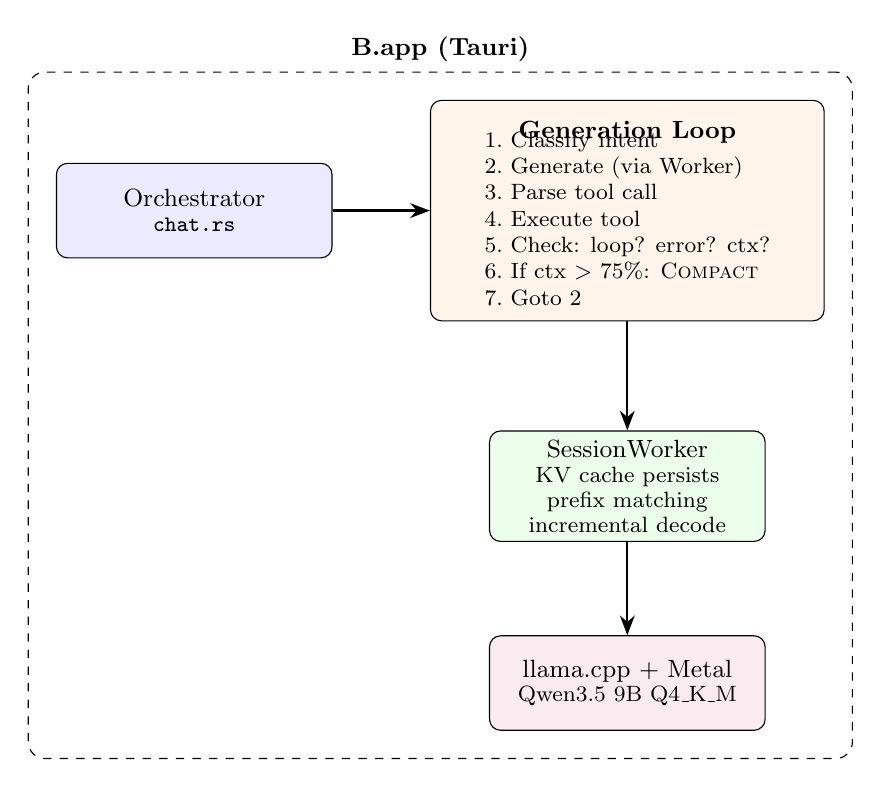
\begin{tikzpicture}[
  box/.style={draw, rounded corners=4pt, minimum width=3.5cm, minimum height=1.2cm, align=center, font=\small},
  bigbox/.style={draw, rounded corners=6pt, dashed, inner sep=10pt},
  arr/.style={-{Stealth[length=2.5mm]}, thick},
]
  % Orchestrator
  \node[box, fill=blue!8] (orch) at (0, 0) {Orchestrator\\[-2pt]\footnotesize\texttt{chat.rs}};

  % Generation loop
  \node[box, fill=orange!8, minimum width=5cm, minimum height=2.8cm] (loop) at (5.5, 0) {};
  \node[font=\small\bfseries] at (5.5, 1.0) {Generation Loop};
  \node[font=\footnotesize, align=left] at (5.5, -0.1) {
    1.~Classify intent\\
    2.~Generate (via Worker)\\
    3.~Parse tool call\\
    4.~Execute tool\\
    5.~Check: loop? error? ctx?\\
    6.~If ctx $>$ 75\%: \textsc{Compact}\\
    7.~Goto 2
  };

  % SessionWorker
  \node[box, fill=green!8] (worker) at (5.5, -3.5) {SessionWorker\\[-2pt]\footnotesize KV cache persists\\[-2pt]\footnotesize prefix matching\\[-2pt]\footnotesize incremental decode};

  % llama.cpp
  \node[box, fill=purple!8] (llama) at (5.5, -6.0) {llama.cpp + Metal\\[-2pt]\footnotesize Qwen3.5 9B Q4\_K\_M};

  % Tauri shell
  \node[bigbox, fit=(orch)(loop)(worker)(llama), label={[font=\small\bfseries]above:B.app (Tauri)}] {};

  % Arrows
  \draw[arr] (orch) -- (loop);
  \draw[arr] (loop) -- (worker);
  \draw[arr] (worker) -- (llama);
\end{tikzpicture}
\caption{System architecture. The orchestrator drives a dynamic generation loop. The SessionWorker persists the KV cache across rounds on a dedicated thread. llama.cpp provides Metal-accelerated inference.}
\label{fig:arch}
\end{figure}

% ══════════════════════════════════════════════════════════════════════
\section{The Forgetting Inequality}

Let $C$ be the context window size, $S$ the system prompt size, $Q$ the user question size, $R_i$ the token count of the $i$-th tool round-trip, and $G$ the generation budget. The model can operate reliably while:

\begin{equation}
S + Q + \sum_{i} R_i + G < C
\label{eq:budget}
\end{equation}

\noindent Without measured forgetting, $\sum_{i} R_i$ grows monotonically and eventually violates the inequality. With measured forgetting, when the sum approaches $T_{\text{compact}}$, the compressible zone is replaced by a summary of size $\sigma$:

\begin{equation}
S + Q + \sigma + R_{\text{recent}} + G < C
\label{eq:compact}
\end{equation}

\noindent where $\sigma \leq 256$ tokens and $R_{\text{recent}}$ covers only the last 2 messages. The inequality is restored and the generation loop continues.

The compression ratio achieved is:

\begin{equation}
\rho = \frac{\sigma}{\sum_{i} R_i} \quad \text{(for compressible rounds)}
\label{eq:ratio}
\end{equation}

\noindent In practice, we observe $\rho \approx 0.03$--$0.08$ --- a 12--33$\times$ compression factor. This is consistent with the high redundancy of multi-round tool exchanges, where each round's prompt re-states context established in prior rounds.

% ══════════════════════════════════════════════════════════════════════
\section{Production Trace: Annotated Case Study}
\label{sec:trace}

The following is a lightly edited trace from B.app (Qwen3 8B, M4 Mac) during a real multi-tool investigation. The user asked: ``What's the current price of GBPUSD and what was the 24h change?'' The model dispatched tool calls to a forex API.

\begin{small}
\begin{verbatim}
Round 1: [tool_call] check_price("GBPUSD")
         [tool_result] {"bid":1.3342,"ask":1.3344,"time":"14:32"}
Round 2: [tool_call] check_candles("GBPUSD","H1",24)
         [tool_result] [{"o":1.3298,"h":1.3356,"l":1.3291,...},
                        ...24 candle objects, ~2100 tokens...]
Round 3: [assistant] Interprets: GBPUSD at 1.3342, 24h open
         was 1.3298, change = +0.0044 (+0.33%).
Round 4: [tool_call] oanda_sentiment("GBPUSD")
         [tool_result] {"long_pct":38.2,"short_pct":61.8}
Round 5: [assistant] Adds sentiment context to answer.
----- context utilisation: 11,847 / 12,288 (96%) -----
----- COMPACTION FIRES -----
\end{verbatim}
\end{small}

\noindent At round 5, context crosses the 75\% threshold (Eq.~\ref{eq:threshold}). The v2 algorithm analyses the 5 intermediate messages:

\begin{small}
\begin{verbatim}
Message scores (Influence Equation):
  Round 1 result: I=4.2 (data+entity+task: 3 dims, Phi=5.2)
  Round 2 result: I=1.8 (data only: 1 dim, Phi=1.0)  ← 2100 tokens
  Round 3 assist: I=6.1 (data+causal+task+temporal: 4 dims, Phi=8.0)
  Round 4 result: I=2.3 (data+entity: 2 dims, Phi=2.8)
  Round 5 assist: I=3.9 (data+causal+task: 3 dims, Phi=5.2)

Tier assignment:
  Tier 1 (verbatim): Round 3 (interpretation with price+change)
  Tier 2 (summarise): Rounds 1, 4, 5
  Tier 3 (heavy compress): Round 2 (24 candles -> "24h range 1.3291-1.3356")
\end{verbatim}
\end{small}

\noindent \textbf{V1 outcome:} All 5 messages fed equally to summariser. The summary mentions ``GBPUSD around 1.33'' but loses the exact bid/ask spread, the 24h open price, and the sentiment split. Post-compaction probe: ``What was the 24h change?'' $\to$ ``approximately 0.3\%'' (score: 2, correct but vague).

\textbf{V2 outcome:} Round 3 (the interpretation) preserved verbatim. Round 2 (the 2100-token candle array) collapsed to one line. Summariser receives 60\% less text but the key numbers survive intact. Post-compaction probe: ``What was the 24h change?'' $\to$ ``+0.0044 (+0.33\%), open 1.3298, current 1.3342'' (score: 3, correct with specifics).

\noindent The compacted context is 3,200 tokens (from 11,847) --- a 73\% reduction. The model continues with a fresh budget, and KV persistence means only the restructured portion needs re-decoding (the 2,400-token system prompt + question prefix is cached).

% ══════════════════════════════════════════════════════════════════════

\begin{thebibliography}{99}
\bibitem{packer2023memgpt}
C.~Packer, S.~Wooders, K.~Lin, V.~Fang, S.\,G.~Patil, I.~Stoica, and J.\,E.~Gonzalez.
\newblock {MemGPT}: Towards {LLM}s as Operating Systems.
\newblock \emph{arXiv preprint arXiv:2310.08560}, 2023.

\bibitem{snell2024scaling}
C.~Snell, J.~Lee, K.~Xu, and A.~Kumar.
\newblock Scaling {LLM} Test-Time Compute Optimally can be More Effective than Scaling Model Parameters.
\newblock \emph{arXiv preprint arXiv:2408.03314}, 2024.

\bibitem{xiao2023streaming}
G.~Xiao, Y.~Tian, B.~Chen, S.~Han, and M.~Lewis.
\newblock Efficient Streaming Language Models with Attention Sinks.
\newblock \emph{arXiv preprint arXiv:2309.17453}, 2023.

\bibitem{jiang2023llmlingua}
H.~Jiang, Q.~Wu, C.-Y.~Lin, Y.~Yang, and L.~Qiu.
\newblock {LLMLingua}: Compressing Prompts for Accelerated Inference of Large Language Models.
\newblock \emph{arXiv preprint arXiv:2310.05736}, 2023.

\bibitem{jiang2024longllmlingua}
H.~Jiang, Q.~Wu, X.~Luo, D.~Li, C.-Y.~Lin, Y.~Yang, and L.~Qiu.
\newblock {LongLLMLingua}: Accelerating and Enhancing {LLM}s in Long Context Scenarios via Prompt Compression.
\newblock \emph{arXiv preprint arXiv:2310.06839}, 2024.

\bibitem{chevalier2023autocompressors}
A.~Chevalier, A.~Wettig, A.~Ajith, and D.~Chen.
\newblock Adapting Language Models to Compress Contexts.
\newblock \emph{arXiv preprint arXiv:2305.14788}, 2023.

\bibitem{mu2024gisting}
J.~Mu, X.\,L.~Li, and N.~Goodman.
\newblock Learning to Compress Prompts with Gist Tokens.
\newblock \emph{NeurIPS}, 2023.

\bibitem{li2023selective}
Y.~Li, B.~Dong, F.~Guerin, and C.~Lin.
\newblock Compressing Context to Enhance Inference Efficiency of Large Language Models.
\newblock \emph{Proceedings of EMNLP}, pages 6342--6353, 2023.

\bibitem{verma2026focus}
N.~Verma.
\newblock Active Context Compression: Autonomous Memory Management in {LLM} Agents.
\newblock \emph{arXiv preprint arXiv:2601.07190}, 2026.

\bibitem{shkolnikov2026kv}
Y.\,P.~Shkolnikov.
\newblock Agent Memory Below the Prompt: Persistent {Q4} {KV} Cache for Multi-Agent {LLM} Inference on Edge Devices.
\newblock \emph{arXiv preprint arXiv:2603.04428}, 2026.

\bibitem{kang2025acon}
M.~Kang, W.-N.~Chen, D.~Han, H.\,A.~Inan, L.~Wutschitz, Y.~Chen, R.~Sim, and S.~Rajmohan.
\newblock {ACON}: Optimizing Context Compression for Long-horizon {LLM} Agents.
\newblock \emph{arXiv preprint arXiv:2510.00615}, 2025.

\bibitem{llamacpp}
G.~Gerganov et al.
\newblock llama.cpp, 2023--2026.
\newblock \url{https://github.com/ggerganov/llama.cpp}.
\end{thebibliography}

\end{document}
